
%-----------------------------------------------------------------------
\begin{figure*}[!t]
  \begin{center}
  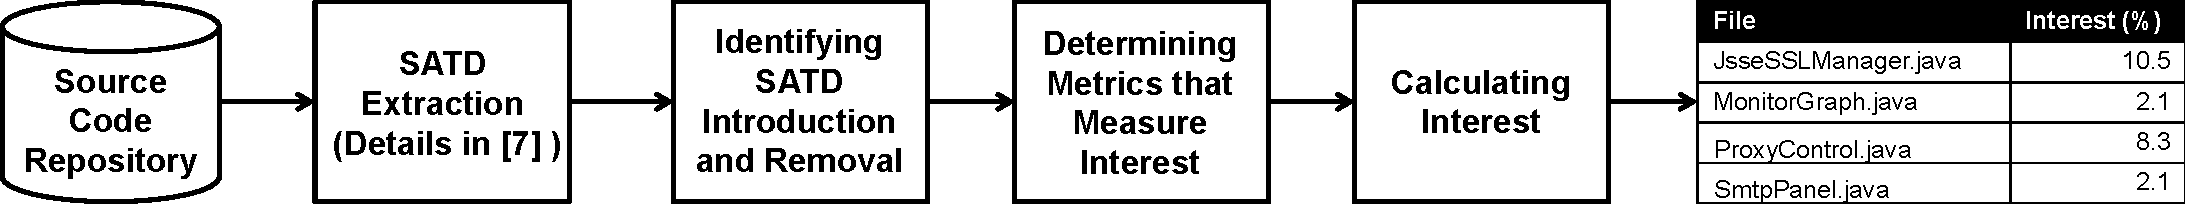
\includegraphics[width=.95\textwidth]{figures/overview}
  \caption{The overview of our approach.}
  \label{fig:overview}
  \end{center}
\end{figure*}
%-----------------------------------------------------------------------


%\section{Case Study Setup} \label{sec:setup}
\section{Approach} \label{sec:approach}
To perform our study, we need to determine the SATD in the codebase, locate when the SATD was introduced in the project and when it was later removed. Then, we use our measures of interest, i.e., LOC and Fan-In, to compare the size of the code and the amount of dependence other code had on the TD code in order to quantify interest (Figure \ref{fig:overview}).

\if0
% Yasu: We just out this part for a position paper.
\subsection{SATD Extraction}
\smallsection{(Step 1) Extract source code files}
To perform our case study, we obtain source code files from Git repositories of three projects. We selected {\sc 1.4.0}, {\sc ANT\_170}, and {\sc v2\_10} in each JRuby, Apache Ant, and Apache jmeter as versions (tags) of which we extract SATD. The versions were released at the middle of project history. Therefore, we believe that projects elapse sufficient time for obtaining technical debt for our analysis and remain time for removing it.

\smallsection{(Step 2) Parse source code files}
After obtaining source code files, we extract the comments from them. We use JDeodorant~\cite{Tsantalis2008CSMR}, which is an open-source Eclipse plug-in, to parse the source code and extract the code comments. JDeodrant uses the Eclipse AST framework to create an Abstract Syntax Tree (AST) map of the source code. The AST map contains detailed information about the project such as: the source code comments, its type (e.g., Block, Single-line, or Javadoc), the line where each one of these comments begins and finishes. We extract the aforementioned information and store all comments as the candidate of SATD.

\smallsection{(Step 3) Filter Comments}
To reduce the number of comments we manually read, we filter comments that are less likely to be classified as SATD by utilizing several heuristics, similar to previous studies~\cite{Maldonado2015MTD}.

First, we eliminate license comments from the candidate of SATD, since we found that license comments are not likely to contain SATD. License comments are commonly added before the declaration of the class. Since we know the line number that the class was declared, we can easily check for comments that are placed before that line and remove them. In order to decrease the chances of removing a SATD comment while executing this filter, we do not remove comments containing one of task-reserved words (i.e., “todo”, “fixme”, or “xxx”).

Then, we also filter Javadoc comments from the candidate of SATD, since we found that they rarely mention SATD. Based on source code comments' type provided by JDeodrant, we identify Javadoc comments. Similar to the heuristics for license comments, we do not remove Javadoc comments containing at least one of task-reserved words. To do so, we create a simple regular expression that search for the task-reserved words before removing the comment.

Then, we group consecutive single-line comments as one comment. We notice that developers sometimes make long comments, using multiple single-line comments instead of a Block comment. This characteristic can hinder the understanding of the message. When considering the case that we analyze each one of these comments independently, we may misunderstand the message because each of them would be incomplete and lose the meaning.

Finally, we filter the comments that conduct {\it comment out} source code from the candidate of SATD. While commented source code may show the code that is currently not being used or the code that was used for debugging, it may not include any developer's comments. Therefore, the commented source code is less likely to be classified as SATD. We remove commented source code using a simple regular expression that captures typical Java code structures.

Table xxx shows the number of comments that are filtered by the heuristics we used. The heuristics significantly reduces the number of comments in our dataset and helps us focus on the most applicable and insightful comments. 

\todo{add a table that shows the number of comments that are filtered by several heuristics}

\smallsection{(Step 4) Manual Classification}
To extract SATD, the xxx author manually classified all comments into SATD or not.
The xxx author who made the classification has more than 8 years of experience working in the industry as a software engineer, during this time he designed, implemented and maintained several programs using, in particular the Java programming language. He developed solid skills in object orientated programming and design patterns. We consider that these qualifications provide the necessary background to conduct the manual classification of the comments.
\fi

%\subsection{Interest Extraction} \label{subsec:interest}

\smallsection{1. SATD Extraction}
In order to measure interest of the TD, our first step is to identify where it exists. Since we focus particularly on SATD, we use code comments found in the source code. We extract and parse the source code of JMeter version 2.10. To perform the parsing, we use the {\sc JDeodorant} tool~\cite{Tsantalis2008CSMR}, which allows us to extract a comment and map it to its corresponding method. Then, we apply a series of filters to remove irrelevant comments, e.g., copyright-related comments. Finally, the 2nd author\footnote{The 2nd author who made the classification has more than 8 years of experience working in the industry as a software engineer, during this time he designed, implemented and maintained several programs using, in particular the Java programming language.} manually classified all comments to determine if they are SATD comments or not and mapped these comments to their respective methods. \revised{In this study, we assume that SATD exists in the method where the comment is identified.} Details regarding the dataset and the filtering applied can be found in our earlier work~\cite{Maldonado2015MTD}.


%To extract SATD, we extract source code files for a version control system. Then we extract the comments from them using JDeodorant~\cite{Tsantalis2008CSMR}, which is an open-source Eclipse plug-in, to parse the source code and extract the code comments.
%To reduce the number of comments we manually read, we filter comments that are less likely to be classified as SATD by utilizing several heuristics, similar to previous studies~\cite{Maldonado2015MTD}. Finally, the 2nd author\footnote{The 2nd author who made the classification has more than 8 years of experience working in the industry as a software engineer, during this time he designed, implemented and maintained several programs using, in particular the Java programming language.} manually classified all comments into SATD or not. See the details of the Step 1 in Maldonado and Shihab's study~\cite{Maldonado2015MTD}.


% \todo{We need to ask Everton about git commonds to find where it was introduced and removed.
\smallsection{2. Identifying SATD Introduction and Removal}
Since we are interested in measuring the interest, we need to determine the `change' over time in these SATD methods. For each of the SATD comments identified by us, we use several git commands (e.g., {\tt git log -- <PATH\_TO\_FILE>} and {\tt git cat-file <SHA1>:<PATH\_TO\_FILE>}), to trace a comment back to the commit where it was introduced. We perform this task by replaying the history commit-by-commit. Using the same technique, we are also able to detect the removal of SATD. \revised{We detect the removal of SATD when we find that the commit is removed or changed.} 
%@Yasu (from Emad's call) we extract all files in versions, and check whether or not SATD is included from the first version of each file to know SATD introduction. Similar to this, we check whether or not SATD is excluded to know SATD removal. 

%@Yasu I commented out the following sentenses since they are almost similar with the above sentenses
%By tracing the comments including SATD across versions in Git repositories, we identify two versions that introduce and remove them. To trace the comments, we obtain patches between two versions over all versions for each file that includes technical debt. Then, we check each patch about whether or not technical debt is introduced and removed. \todo{Need to merge the prior 2 sentences}

\smallsection{3. Determining Metrics that Measure Interest}
Once we are able to determine the SATD comments and their associated methods, we would like to calculate the interest that is incurred over time (i.e., from the introduction of the technical debt to its removal). To do so, we extracted 16 code metrics using the {\sc Understand Tool}~\cite{Understand}. In particular, we selected all method-level complexity and size metrics that Understand is able to provide.

The reasons that we focused on complexity and size metrics are: 1) our intuition tells us that if a piece of code is introduced and then becomes more complex, then that is a good proxy for it being more difficult to deal with in the future, i.e., it incurred interest; and 2) prior work has shown that size metrics are typically highly correlated with complexity metrics, hence, we figured using size metrics (if they are highly correlated with complexity metrics in our case) would be an easier alternative to using complexity metrics.

We performed the \revised{Spearman's} correlation analysis between the complexity and size metrics and found that indeed all metrics except Fan-In are highly correlated with LOC. Therefore, we decided to use the LOC metric as a measure of interest. In addition, since Fan-In is an indicator of how much a method is depended on, we decided to also include the Fan-In metric when calculating interest. The intuition being that if a method is depended on lightly when the SATD is introduced and then has many more dependencies in the future, then dealing with this SATD is much more difficult (since many dependencies may be affected). In the end, we settled on using the two metrics, LOC and Fan-In, as measures of interest.

%To calculate interest, we measure product metrics from two versions detected in Step 2 using {\sc Understand}~\cite{Understand}. We choose all metrics (e.g., LOC and Cyclymatic Complexity) that are available at the method-level in {\sc Understand}.

\smallsection{4. Calculating Interest}
Using our metrics, we consider the relative LOC and Fan-In  values between the introduced and removed versions as interest. For example, if arbitrary metric values in the introduced and removed versions are 10 and 20, the relative size is 50 (i.e, $100* \frac{(20-10)}{20}$). In cases where the SATD is not yet removed, we use the numbers from the latest version of JMeter.

\revised{If the SATD incurs a positive interest rate, it would have additional difficulty to be removed. We consider that when the SATD becomes more complex, then that becomes more difficult to deal with it.}

While the paper tackles the research topic that accelerates a new research direction (i.e., quantifying interest of SATD), it also has the weakness of our current approach. We elaborate on the weakness of our current approach in Section \ref{conclusion}.


\begin{figure*}[!t]
  \begin{center}
  \scalebox{0.95}{
  \begin{tabular}{cc}
    \subfigure[JMeter (LOC)]{ 
      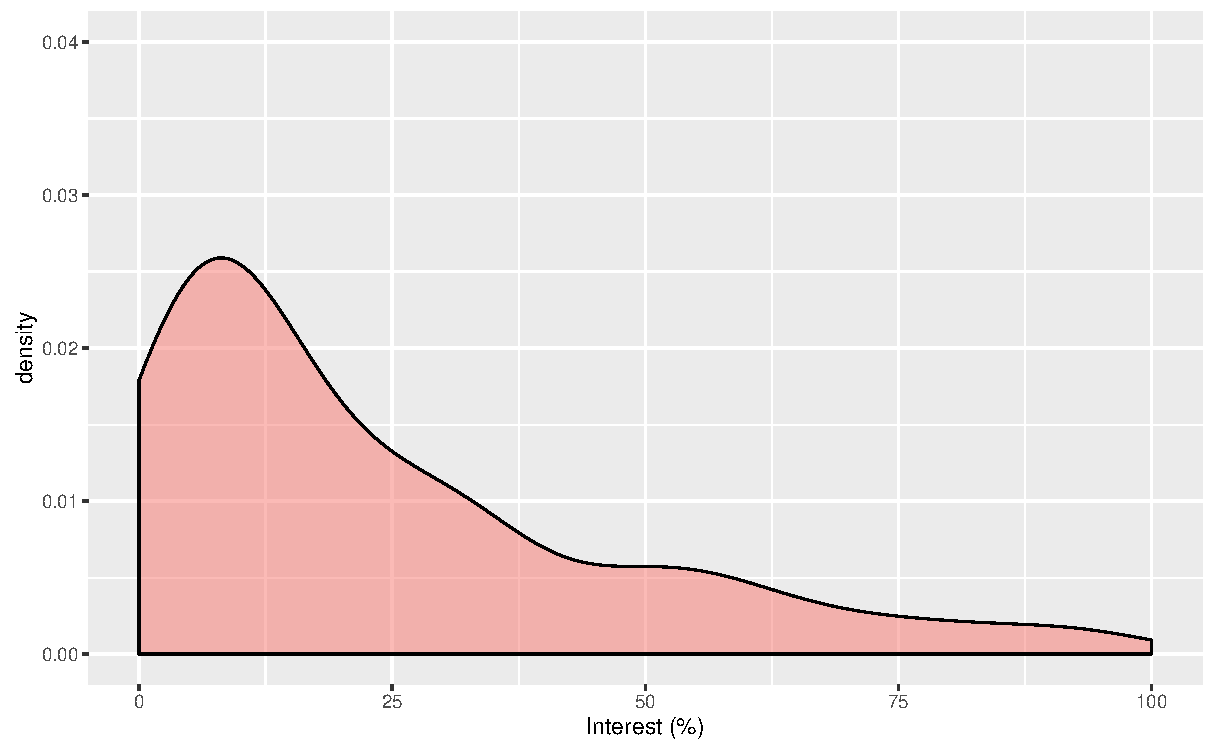
\includegraphics[width=.45\textwidth]{figures/rq1-jmeter}
    }
    \subfigure[JMeter (Fan-In)]{ 
      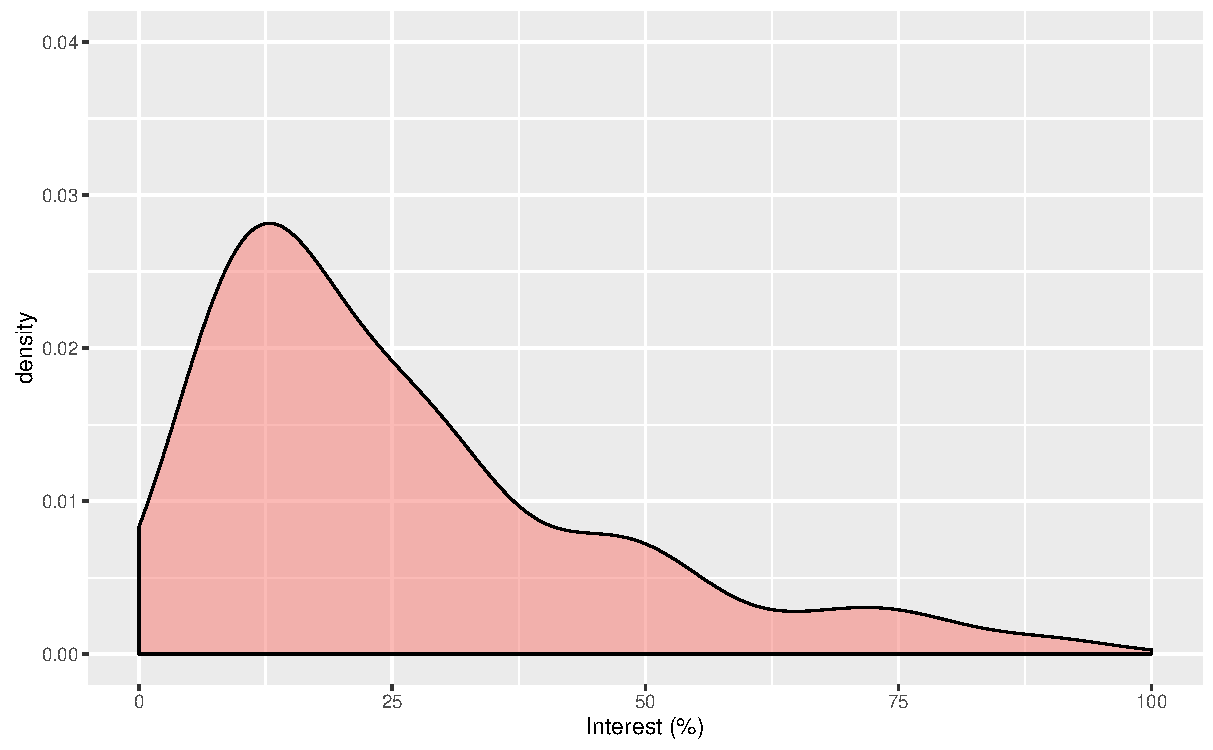
\includegraphics[width=.45\textwidth]{figures/rq1-jmeter-fanin}
    }
  \end{tabular}
  }

  \caption{The results of distribution of interest.}
  \label{fig:dist}
  \end{center}
\end{figure*}
